\section{Framework Structure}
\label{sec:framework}
In order to assess Atlas' aptitude as a censorship measurement platform, we continue by presenting \textsf{Cartography}, our framework based on RIPE Atlas.

\subsection{RIPE Atlas Background}
% Some basic information about Atlas.
Having been founded in 2010 by RIPE NCC, Atlas~\cite{atlas} is a globally
distributed Internet measurement network consisting of physical probes hosted by
volunteers.  Once a user connects her probe to the network, it can be used by other participants for outbound measurements. So-called \emph{credits} are awarded
automatically based on the uptime of contributed probes, which are expended in order to perform custom measurements. Queries to probes can be initialized centrally either over the web frontend, or over a RESTful API.

% Geographic and topological distribution.
An ideal censorship measurement platform features high geographic and
topological diversity, thereby facilitating measurements in any region where
censorship occurs.  While Atlas probes are distributed throughout the world,
there is a significant bias towards the U.S. and Europe as can be seen in
Figure~\ref{fig:probe_distribution}.  As for Atlas' topography, only 68
autonomous systems contain 40\% of all Atlas probes with the three most common
autonomous systems being 7922 (4.4\%, Comcast Cable Communications), 3320
(3.2\%, Deutsche Telekom), and 6830 (2.8\%, Liberty Global Operations).  While
not optimal, most censoring regions still contain at least several probes.

\begin{figure}[t]
\centering
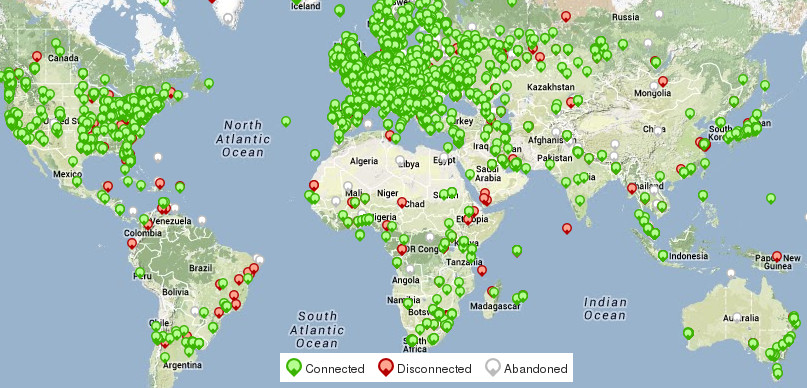
\includegraphics[width=0.48\textwidth]{diagrams/probe_distribution.jpg}
\caption{The geographic distribution of Atlas probes as of May 2014.  Green
icons represent active probes and red icons represent probes which are
currently offline.  The distribution is biased towards the U.S. and Europe.}
\label{fig:probe_distribution}
\end{figure}

% What kind of measurements does Atlas allow?
As of May 2014, Atlas allows four types of measurements; ping, traceroute, DNS
resolution, and X.509 certificate fetching (labeled SSLCert).  All four measurement types can
further be parameterized for more fine-grained control.  HTTP requests are not
possible at this point due to abuse and security concerns.  While Atlas clearly lacks the
flexibility of comparable platforms (see Table~\ref{tab:comparison}), it makes
up for it with comparably high diversity, responsiveness and continued growth.  After all,
we do not expect Atlas to replace existing platforms, such as OONI, but rather to
\emph{complement} them.

% TODO - Should we talk about our crappy command-line interface?

% We also need to mention how you can stablish a big experiments using RIPE.
% And mention about the propblem of how you frist need to submit your
% experiments and then it will give you predicted cost. This way we can move to
% cost function.

\subsection{Atlas Cost Model}

As briefly mentioned above, Atlas' measurement have to be paid with credits.  The exact ``price'' of a measurement depends on the
measurement type, its parameters, and the destination(s).  The credit system
works based on a linear cost model.  Each user has a credit balance that can be
increased by hosting Atlas probes, or by receiving credits from other users.

Table~\ref{tab:cost} list the currently available measurement types as well as
their associated costs.  While DNS and SSLCert measurements have a fixed cost,
ping and traceroutes vary depending on the amount and sizes of packets.  Also,
the atomic cost of one-off measurements are twice as much as the one of repeated
measurements.  When scheduling a new experiment, the user first specifies the
details (e.g., measurement type as well as measurement parameters).  Afterwards, the
Atlas web-based frontend calculates the measurement costs on the server side and
shows it to the user.  Finally, upon completion of the measurement, the
respective cost is subtracted from the user's credit balance.

Due do the non-deterministic nature of pings and traceroutes, and measurements
in general, we developed a command-line based tool to help users create new
measurements and estimate their costs.  As input, the tool expects \emph{1)} a
country of interest, \emph{2)} the amount of credits, the user is willing to
``pay'', and \emph{3)} a measurement type.  Our tool then determines the amount
of available probes (if any), the expected costs, and runs the measurement if
the cost is below the user's expected cost.

%\subsection{Calculating Costs}
%
%Predicted cost = $\sum_{i=1}^{5} (C_i * N_i)$  where i can be (DNS, SSL, ...)\\
%Remaining credits = min(available cost, desired cost) - predicted cost
%
%Note that it is a linear cost model so number of probs included doesn't matter
%in the cost part it matters when we suggest the experiment by just uniformly
%distribute the possible number of measurements on one(total experiments
%possible/Num probs)
%This should be included in the API philipp wrote (TODO)
%
%one-off measurements cost twice as much as not one-off.

% \subsection{Evaluation of our cost model}
% To test that our cost prediction is accurate, we ran a series of unit cost with
% different values, and compared  the suggested cost and the actual credit
% subtracted with the cost our approach suggest. Because the number of possible
% cases are finite we can run all unit measurements, then calculate confidence
% interval to show how good we do.
% 
% We choose a prob(12214) 

\begin{table}[ht!]
\centering
\begin{tabular}{lc}
\hline
\textbf{Unit Measurement} & \textbf{Cost} \\
\hline 
DNS\slash DNS6 (TCP) & 20\\ 
DNS\slash DNS6 (UDP) & 10\\ 
SSLCert\slash SSLCert6 & 10 \\
Ping\slash Ping6 & $N * (int(S/1500)+1)$\\
Traceroute\slash Traceroute6 & $ 10*N*(int(S/1500)+1)$\\[1ex] 
\hline 
\end{tabular} 
\caption{The cost model for Atlas measurements.  The variable $N$ refers to the
number of packets whereas the variable $S$ refers to packet sizes.  Note that
the cost for TCP-based DNS measurement differs for UDP-based measurements.}
\label{tab:cost} 
\end{table}

\subsection{Ethical Aspects}
% The problem.
Atlas was not designed as censorship analysis platform and accordingly, its
volunteers likely do not expect that their probes will be used for such
purposes.  Careless measurements could attract a censor's attention and cause
repercussions for the respective probe operator.

However, Atlas' measurement types are limited to ping, traceroute, DNS requests
and X.509 certificate fetching.  As of May 2014, it is not possible to create
HTTP requests or engage in actual, meaningful communication with arbitrary
destinations, which limits the damage caused by reckless measurement.
Nevertheless, we acknowledge that care must be taken and hope to initiate
further ethical discussions that would inform broader measurement efforts.

For a more comprehensive ethical discussion, refer to Wright et
al.~\cite[\S~5]{Wright2011}.
